%!TEX program = xelatex+makeindex+bibtex
\documentclass[final]{scrreprt} %scrreprt of scrartcl
% Include all project wide packages here.
\usepackage{fullpage}
\usepackage{polyglossia}
\setmainlanguage{english}
\usepackage{csquotes}
\usepackage{graphicx}
\usepackage{epstopdf}
\usepackage{pdfpages}
\usepackage{caption}
\usepackage[list=true]{subcaption}
\usepackage{float}
\usepackage{standalone}
\usepackage{import}
\usepackage{tocloft}
\usepackage{wrapfig}
\usepackage{authblk}
\usepackage{array}
\usepackage{booktabs}
\usepackage[toc,page,title,titletoc]{appendix}
\usepackage{xunicode}
\usepackage{fontspec}
\usepackage{pgfplots}
\usepackage{SIunits}
\usepackage{units}
\pgfplotsset{compat=newest}
\pgfplotsset{plot coordinates/math parser=false}
\newlength\figureheight 
\newlength\figurewidth
\usepackage{amsmath}
\usepackage{mathtools}
\usepackage{unicode-math}
\usepackage[
    backend=bibtexu,
	texencoding=utf8,
bibencoding=utf8,
    style=ieee,
    sortlocale=en_US,
    language=auto
]{biblatex}
\usepackage{listings}
\newcommand{\includecode}[3][c]{\lstinputlisting[caption=#2, escapechar=, style=#1]{#3}}
\newcommand{\superscript}[1]{\ensuremath{^{\textrm{#1}}}}
\newcommand{\subscript}[1]{\ensuremath{_{\textrm{#1}}}}


\newcommand{\chapternumber}{\thechapter}
\renewcommand{\appendixname}{Bijlage}
\renewcommand{\appendixtocname}{Bijlagen}
\renewcommand{\appendixpagename}{Bijlagen}

\usepackage[hidelinks]{hyperref} %<--------ALTIJD ALS LAATSTE

\renewcommand{\familydefault}{\sfdefault}

\setmainfont[Ligatures=TeX]{Myriad Pro}
\setmathfont{Asana Math}
\setmonofont{Lucida Console}

\usepackage{titlesec, blindtext, color}
\definecolor{gray75}{gray}{0.75}
\newcommand{\hsp}{\hspace{20pt}}
\titleformat{\chapter}[hang]{\Huge\bfseries}{\chapternumber\hsp\textcolor{gray75}{|}\hsp}{0pt}{\Huge\bfseries}
\renewcommand{\familydefault}{\sfdefault}
\renewcommand{\arraystretch}{1.2}
\setlength\parindent{0pt}

%For code listings
\definecolor{black}{rgb}{0,0,0}
\definecolor{browntags}{rgb}{0.65,0.1,0.1}
\definecolor{bluestrings}{rgb}{0,0,1}
\definecolor{graycomments}{rgb}{0.4,0.4,0.4}
\definecolor{redkeywords}{rgb}{1,0,0}
\definecolor{bluekeywords}{rgb}{0.13,0.13,0.8}
\definecolor{greencomments}{rgb}{0,0.5,0}
\definecolor{redstrings}{rgb}{0.9,0,0}
\definecolor{purpleidentifiers}{rgb}{0.01,0,0.01}


\lstdefinestyle{csharp}{
language=[Sharp]C,
showspaces=false,
showtabs=false,
breaklines=true,
showstringspaces=false,
breakatwhitespace=true,
escapeinside={(*@}{@*)},
columns=fullflexible,
commentstyle=\color{greencomments},
keywordstyle=\color{bluekeywords}\bfseries,
stringstyle=\color{redstrings},
identifierstyle=\color{purpleidentifiers},
basicstyle=\ttfamily\small}

\lstdefinestyle{c}{
language=C,
showspaces=false,
showtabs=false,
breaklines=true,
showstringspaces=false,
breakatwhitespace=true,
escapeinside={(*@}{@*)},
columns=fullflexible,
commentstyle=\color{greencomments},
keywordstyle=\color{bluekeywords}\bfseries,
stringstyle=\color{redstrings},
identifierstyle=\color{purpleidentifiers},
}

\lstdefinestyle{matlab}{
language=Matlab,
showspaces=false,
showtabs=false,
breaklines=true,
showstringspaces=false,
breakatwhitespace=true,
escapeinside={(*@}{@*)},
columns=fullflexible,
commentstyle=\color{greencomments},
keywordstyle=\color{bluekeywords}\bfseries,
stringstyle=\color{redstrings},
identifierstyle=\color{purpleidentifiers}
}

\lstdefinestyle{vhdl}{
language=VHDL,
showspaces=false,
showtabs=false,
breaklines=true,
showstringspaces=false,
breakatwhitespace=true,
escapeinside={(*@}{@*)},
columns=fullflexible,
commentstyle=\color{greencomments},
keywordstyle=\color{bluekeywords}\bfseries,
stringstyle=\color{redstrings},
identifierstyle=\color{purpleidentifiers}
}

\lstdefinestyle{xaml}{
language=XML,
showspaces=false,
showtabs=false,
breaklines=true,
showstringspaces=false,
breakatwhitespace=true,
escapeinside={(*@}{@*)},
columns=fullflexible,
commentstyle=\color{greencomments},
keywordstyle=\color{redkeywords},
stringstyle=\color{bluestrings},
tagstyle=\color{browntags},
morestring=[b]",
  morecomment=[s]{<?}{?>},
  morekeywords={xmlns,version,typex:AsyncRecords,x:Arguments,x:Boolean,x:Byte,x:Char,x:Class,x:ClassAttributes,x:ClassModifier,x:Code,x:ConnectionId,x:Decimal,x:Double,x:FactoryMethod,x:FieldModifier,x:Int16,x:Int32,x:Int64,x:Key,x:Members,x:Name,x:Object,x:Property,x:Shared,x:Single,x:String,x:Subclass,x:SynchronousMode,x:TimeSpan,x:TypeArguments,x:Uid,x:Uri,x:XData,Grid.Column,Grid.ColumnSpan,Click,ClipToBounds,Content,DropDownOpened,FontSize,Foreground,Header,Height,HorizontalAlignment,HorizontalContentAlignment,IsCancel,IsDefault,IsEnabled,IsSelected,Margin,MinHeight,MinWidth,Padding,SnapsToDevicePixels,Target,TextWrapping,Title,VerticalAlignment,VerticalContentAlignment,Width,WindowStartupLocation,Binding,Mode,OneWay,xmlns:x}
}

%defaults
\lstset{
basicstyle=\ttfamily\small,
extendedchars=false,
numbers=left,
numberstyle=\ttfamily\tiny,
stepnumber=1,
tabsize=4,
numbersep=5pt
}
\addbibresource{../../library/bibliography.bib}
\title{Module 1 - Report}
\author{Sander {van Dijk} \and Erwin {de Haan}}
\begin{document}

\chapter{Werking van de overcurrent protection}
In order to wireless charge our car we had to design a DC-DC converter. The DC-DC converter is splitted into two parts, the DC-AC converter and AC-DC converter respectively. For the DC-AC converter see Figure \ref{fig:DC-AC} and for the AC-DC see Figure \ref{fig:AC-DC}

\begin{figure}[h]
	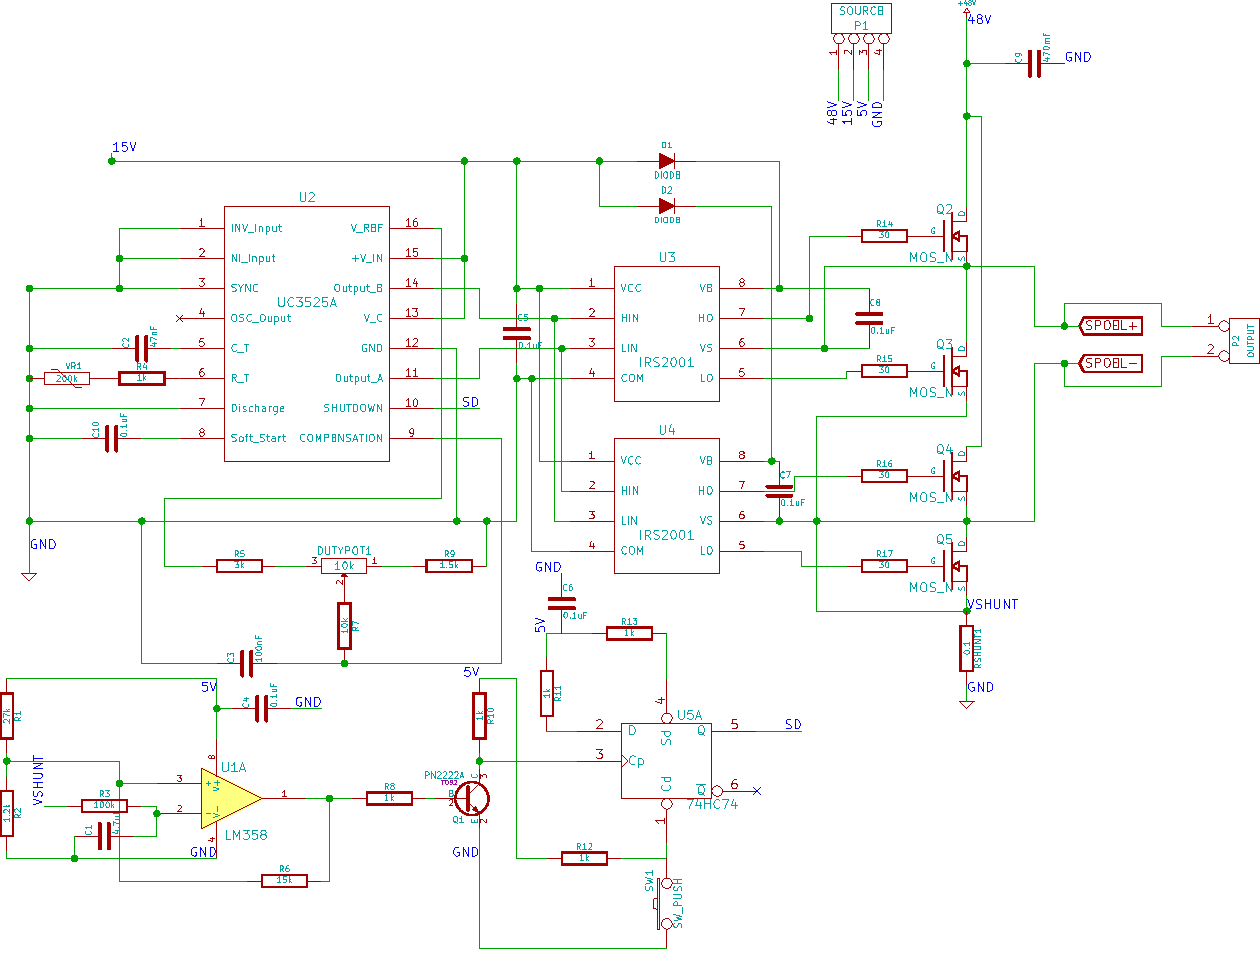
\includegraphics[width=\linewidth]{resources/DC-AC-rc.pdf}
	\caption{DC-AC subcircuit}
	\label{fig:DC-AC}
\end{figure}

\begin{figure}[h]
	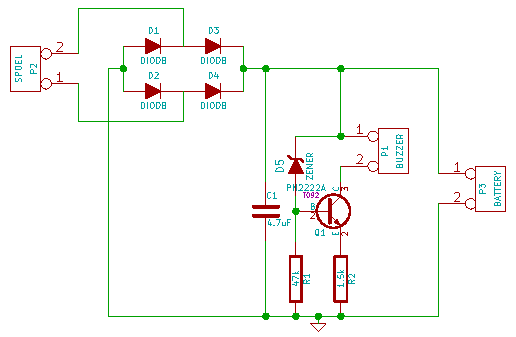
\includegraphics[width=\linewidth]{resources/AC-DC-rc.pdf}
	\caption{AC-DC subcircuit}
	\label{fig:AC-DC}
\end{figure}

For the NMOS transistor used in Figure \ref{fig:DC-AC} we used the IPP028N08N3G (OptiMOS 3) transistor instead of the IPP50CN10N (OptiMOS 2).
We had two reasons for this decision.
\begin{enumerate}
\item First, the drain-source on-state resistance was approximally ten times lower on the OptiMOS 3, causing the transistor to generate less heat and gain better efficiency.
\item Secondly, by looking at the current-voltage characteristics per frequency (\cite{OptiMOS2} \emph{:3 Safe operating area} and \cite{OptiMOS3} \emph{:3 Safe operating area}) we found out that the OptiMOS 3 performs better at higher frequencies than the OptiMOS 2.
\end{enumerate}
We also had to choose the diodes used on the secondary side of the tranformer. The diodes will form a full bridge rectifier, which in combination with a capacitor, will form a AC-DC converter.
The candidates are the SB540 (datasheet: \cite{SB540}) and the SF61 (datasheet: \cite{SF61}).
The forward voltage of the two diodes differ, the SB540's is lower. This is favorable since there will be more voltage left on the output terminals.
On the other hand, the SF61 has a much lower reverse current. Lower reverse current makes the diode more ideal, since it sould only conduct when the current is in forward direction.
We chose the SF61 since we thought the reverse current would be more important.
\\
%After soldering the inverter and rectifier we tested the two parts.
%Figure \ref{fig:AandB} displays the voltage on the output-A and output-B of the UC3525a, which are the oscillating opposites of each other.
%This oscillating pair drives the transistor H-bridge, powering the primary coil.
%The secondary coil will generate a voltage from this primary coil's voltage, which is displayed in Figure \ref{fig:AC_sec}.
%This voltage is rectified using the full bridge rectifier and a small capacitor, it is turned into a DC-voltage as shown in Figure \ref{fig:DC_out}.


The mutual inductance of the two coils can be found by measuring both the opposing and aiding configuration of the coils. The results are given in Table \ref{tab:inductances}.

\begin{table} [h]
\begin{center}
	\begin{tabular}{ l | l | l | l | l }
	Distance & Aiding inductance ($\mu$H) & Opposing inductance ($\mu$H) & Mutual inductance ($\mu$H) & k \\ \hline
  	0 cm & 312.5 & 145.8 & 41.7 & 0.599 \\
	2 cm & 276.0 & 186.4 & 22.4 & 0.322 \\
	4 cm & 258.0 & 199.3 & 14.7 & 0.211 \\
	6 cm & 248.0 & 204.0 & 11.0 & 0.158 \\
	\end{tabular}
	\caption{Inductance in aiding and opposing configuration plus conclusion}
	\label{tab:inductances}
\end{center}
\end{table}

We also measured the resistances of the two coils. The primary coil has a resistance of 0.3 $\Omega$ and the secondary coil has a resistance of 0.1 $\Omega$.
\\
We used the circuit shown in Figure 1.9 of \cite{epo4-manual} to model our circuit. Equation \ref{eq:matrix} was created by applying Kirchhoff's Voltage Law on both current loops.

\begin{equation}
	\begin{bmatrix}
		V_1 \\
		0
	\end{bmatrix} =
	\begin{bmatrix}
		j \omega L_1 + r_1 & -j \omega M \\
		-j \omega M & j \omega L_2 + r_2 + R
	\end{bmatrix}
	\begin{bmatrix}
		I_1 \\
		I_2
	\end{bmatrix}
	\label{eq:matrix}
\end{equation}

\begin{equation}
	\eta = \frac{P_{out}}{P_{in}} = \frac{{I_2}^2 R}{V_1 I_1}
	\label{eq:efficiency}
\end{equation}

Solving Equation \ref{eq:matrix} for $I_1$ and $I_2$ and using them in Equation \ref{eq:efficiency} yields an efficiency of 5.14\% at 2 cm and 1.17\% at 6 cm.
\\ \\
Besides calculating the theoretical efficiency (Equation \ref{eq:efficiency}) we also measured it. Figure \ref{fig:DC_out} displays the result on the oscilloscope, which is approximally 224 mV. Equation \ref{eq:efficiencyMeasured} calculates the efficiency of the DC-DC transformer using this 224 mV. The input of the circuit is measured by the voltage source at 20 V and 0.70 A. The measurement was done with a distance of 2 cm between the coils.

\begin{equation}
	\eta = \frac{P_{out}}{P_{in}} = \frac{{I_2}^2 R_L}{V_1 I_1} = 3.7\%
	\label{eq:efficiencyMeasured}
\end{equation}

We used a different approach from e.g. the iron core transformer for the air core transformer because the mutual inductance is much lower here. Therefore, the short and open circuit test are not accurate for air core transformers.
\\ \\
The mutual inductance is instead determined by using the aiding and opposing inductance. In aiding configuration the two coils add up their own inductance but also the mutual inductance adds up to the total. In opposing configuration the two coils also add up, but the mutual inductance is substracted from the total. This way you can find the mutual inductance by substracting the opposing from the aiding inductance.
\\ \\
When the two coils are moving from each other, the leakage and magnitising current both increase, making the transformer less efficient.
\\ \\
When the transformer is not compensated the primary impedance is very high, making the efficiency and throughput lower. The secondary coil has a higher impedance when not compensated too, also resulting in a lower efficiency.

To simulate the circuit in resonance, the model as in Figure 1.9 of \cite{epo4-manual} has been altered. $L_1$ and $L_2$ were considered to be 0 H, as they were compensated by the capacitors in series. However, the mutual inductance is kept unchanged. As in Assignment 2, a matrix was made by applying Kirchhoff's Voltage Law on both loops. Equation \ref{eq:matrixCompensated} is the result of those equations.

\begin{equation}
	\begin{bmatrix}
		V_1 \\
		0
	\end{bmatrix} =
	\begin{bmatrix}
		 r_1 & -j \omega M \\
		-j \omega M & r_2 + R
	\end{bmatrix}
	\begin{bmatrix}
		I_1 \\
		I_2
	\end{bmatrix}
	\label{eq:matrixCompensated}
\end{equation}

As in Assignment 2, the efficiency of the circuit is calculated from $I_1$ and $I_2$, yielding 93.1\% with the coils 6 cm apart.
\\ \\
The actual efficiency at 6 cm is measured at 71.6\%.
The difference between the calculation and the measurement can be explained by looking at the compensation.
The capacitors we picked were not the exact values as calculated, on both primary and secondary side of the transformer.
Finetuning the frequency can not fix the problem primary and secondary at the same time since the required frequencies differ.
\\ \\
You can test how the air core transformer will react by connecting a 100 kHz sinusoidal voltage because the voltage will be sinusoidal in resonance too.
\\ \\ 
By adding capacitors in series with the coil, the inductance of the coil will be compensated when the capacitance is chosen correctly. Less impedance means a higher current and more power to be transformed. The capacitance can be found from Equation \ref{eq:cap}.

\begin{equation}
	0 = j \omega L + \frac{1}{j \omega C}
	\label{eq:cap}
\end{equation}

When compensated, the coil has only very little resistance left, short circuiting the power source. This high current might damage the circuit, so this should be avoided. This is done with an overcurrent protection.
\\ \\
The overcurrent protection works by measuring the current and turning down the circuit when it becomes too high. The current is measured by placing a low resistant shunt-resistor in series with the coil. The voltage over that resistor is used in a comparator with a fixed compare voltage. When the voltage exceeds the compare voltage, a memory cell is set. Until it is reset, the oscillator is turned down, preventing current flow in the coil.




\chapter{Discussion on the overcurrent protection}
\end{document}